\chapter*{Tarefa - 2}

\section*{Enunciado}

\begin{figure}[h!]
\centering
\caption{Enunciado da Tarefa 2.}
\centering
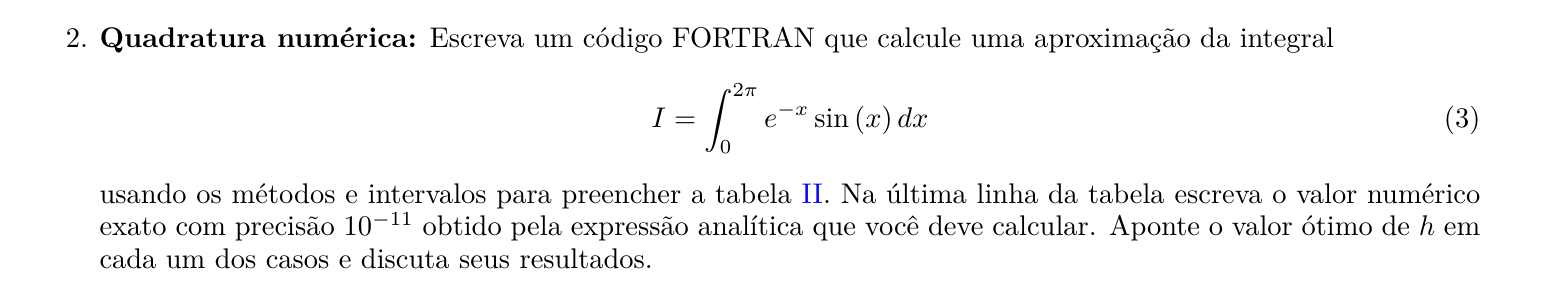
\includegraphics[width=16cm]{images/tarefa-2/enunciado-tarefa-2.png}
\caption*{Fonte: Compilado pelo Autor.}
\label{fig:tarefa 2 - Enunciado}
\end{figure}


\begin{figure}[h!]
\centering
\caption{Tarefa enunciado da Tarefa 2.}
\centering
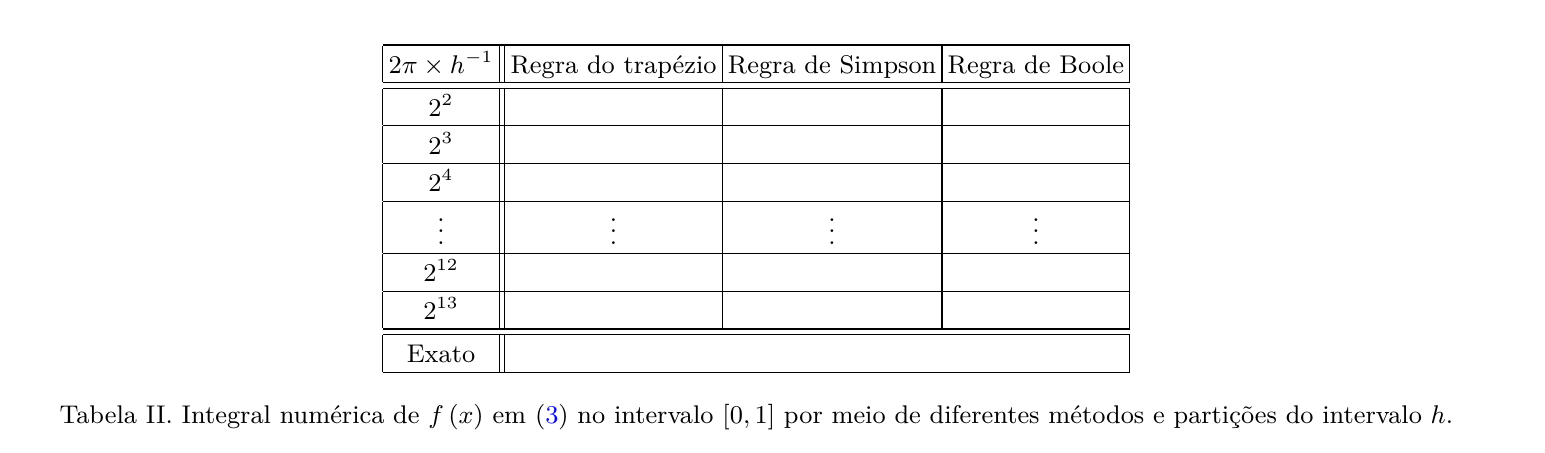
\includegraphics[width=17cm]{images/tarefa-2/tabela-enunciado-tarefa-2.png}
\caption*{Fonte: Compilado pelo Autor.}
\label{fig:tarefa 2 - Tabela Enunciado}
\end{figure}

\section*{Código}


\begin{figure}[H]
\centering
\caption{Função principal do código.}
\centering

\begin{lstlisting}
        program main
        implicit real*8 (a-h,o-z)

C       Constantes

        pi = acos(-1d0)

        a = 0d0
        b = 2d0*pi

C       Variáveis

        rval = 0.5d0*(1d0-exp(-2d0*pi))

        open(unit=1,file='saida-1-12694394.txt')

        do i = 2,13
        n = 2**i
        write(1,7) i,trap(a,b,n),simp(a,b,n),boole(a,b,n)
        end do
        write(1,3) rval
3       format(F16.11)
7       format(I3,3(',',F16.12))
        
        close(1)
        end program main
\end{lstlisting}

\caption*{Fonte: Compilado pelo Autor.}
\label{fig:tarefa 2 - função principal do código}
\end{figure}


\begin{figure}[H]
\centering
\caption{Função principal do código.}
\centering

\begin{lstlisting}
        function f(x)
        implicit real*8 (a-h,o-z)

        f = exp(-x)*sin(x)
        return
        end function f
\end{lstlisting}

\caption*{Fonte: Compilado pelo Autor.}
\label{fig:tarefa 2 - função estudada}
\end{figure}

\begin{figure}[H]
\centering
\caption{Função principal do código.}
\centering

\begin{lstlisting}
        function trap(a,b,n)
        implicit real*8 (a-h,o-z)

        h = (b-a)/n
        trap = 0d0
        do i = 1,n
            x = a + (i-1)*h
            rr = 0.5d0*h*(f(x+h)+f(x))
            trap = trap + rr
        end do

        return
        end function trap
\end{lstlisting}

\caption*{Fonte: Compilado pelo Autor.}
\label{fig:tarefa 2 - função trap}
\end{figure}

\begin{figure}[H]
\centering
\caption{Função principal do código.}
\centering

\begin{lstlisting}
        function boole(a,b,n)
        implicit real*8 (a-h,o-z)


        h = (b-a)/n
        boole = 0d0
        do i = 1,n
        x = a+(i-1)*h
        r1 = (2d0/45d0)*h
        r2 =(7d0*f(x-2d0*h)+7d0*f(x+2d0*h))
        r3 = (32d0*f(x-h)+12*f(x+h)+32d0*f(x+h))

        boole = boole + r1*(r2 + r3)/4d0
        end do

        return
        end function boole
\end{lstlisting}

\caption*{Fonte: Compilado pelo Autor.}
\label{fig:tarefa 2 - função boole}
\end{figure}

\begin{figure}[H]
\centering
\caption{Função principal do código.}
\centering

\begin{lstlisting}
        function simp(a,b,n)
        implicit real*8 (a-h,o-z)


        h = (b-a)/n
        simp = 0d0

        do i = 1,n
        x = a+(i-1)*h
        rr = (3d0*h/8d0)*(f(x)+3d0*f(x+h)+3d0*f(x+2d0*h)+f(x+3d0*h))
        simp = simp + rr/3d0
        end do

        return
        end function simp
\end{lstlisting}

\caption*{Fonte: Compilado pelo Autor.}
\label{fig:tarefa 2 - função simp}
\end{figure}


\section*{Descrição do código}
O programa \texttt{main} tem como objetivo calcular numericamente 
a integral da função

\begin{equation}
	I = \int_{0}^{2\pi}e^{-x} \sin(x)dx
\end{equation}

\noindent 
utilizando diferentes métodos de 
integração numérica: regra do trapézio, regra de Simpson 3/8 e regra de Boole.  
As aproximações são avaliadas para valores de $n = 2^i$, com 
$i = 2,3,\ldots,13$, permitindo analisar a convergência dos métodos 
à medida que o número de subdivisões aumenta.

\bigskip
No início do código, é utilizada a diretiva:

\vspace*{1\baselineskip}
\begin{lstlisting}
implicit real*8 (a-h,o-z)
\end{lstlisting}

\noindent
que define todas as variáveis cujos nomes começam com as letras 
de \textbf{a} a \textbf{h} e \textbf{o} a \textbf{z} como números reais 
de dupla precisão. Em seguida, o programa define constantes:

\vspace*{1\baselineskip}
\begin{lstlisting}
pi = acos(-1d0)
a = 0d0
b = 2d0*pi
\end{lstlisting}

\noindent
e o valor exato para a integral estudada:

\vspace*{1\baselineskip}
\begin{lstlisting}
rval = 0.5d0*(1d0-exp(-2d0*pi))
\end{lstlisting}

\noindent
O arquivo de saída é aberto com o comando:

\vspace*{1\baselineskip}
\begin{lstlisting}
open(unit=1,file='saida-1-12694394.txt')
\end{lstlisting}

\bigskip
No bloco principal, o programa entra em um laço:

\vspace*{1\baselineskip}
\begin{lstlisting}
do i = 2,13
    n = 2**i
    write(1,7) i,trap(a,b,n),simp(a,b,n),boole(a,b,n)
end do
\end{lstlisting}

\noindent
Em cada iteração, $n = 2^i$ define o número de subdivisões, e as funções 
\texttt{trap}, \texttt{simp} e \texttt{boole} calculam a integral usando 
as respectivas regras. Os resultados são escritos no arquivo de saída com o formato:

\vspace*{1\baselineskip}
\begin{lstlisting}
7 format(I3,3(',',F16.12))
\end{lstlisting}

\noindent
Após o laço, o valor de referência \texttt{rval} é escrito no arquivo com o formato:

\vspace*{1\baselineskip}
\begin{lstlisting}
3 format(F16.11)
\end{lstlisting}

\noindent
Por fim, o arquivo é fechado com:

\vspace*{1\baselineskip}
\begin{lstlisting}
close(1)
\end{lstlisting}

\subsection*{Funções auxiliares}

As funções implementam diferentes métodos de integração numérica sobre $[a,b]$.

\begin{enumerate}
    \item \textbf{Função \texttt{f(x)}} \\
    Define a função a ser integrada:
    \begin{equation}
        f(x) = e^{-x} \sin(x)
    \end{equation}

    \item \textbf{Função \texttt{trap(a,b,n)}} — Regra do Trapézio \\
    Aproxima a integral por:
    \begin{equation}
        \int_a^b f(x)\,dx \approx \sum_{i=1}^{n} \frac{h}{2}\Big(f(x_i)+f(x_{i+1})\Big),
    \end{equation}
    onde $h = (b-a)/n$ e $x_i = a + (i-1)h$.

    \item \textbf{Função \texttt{simp(a,b,n)}} — Regra de Simpson 3/8 \\
    Aproximação de quarta ordem que utiliza quatro pontos por subintervalo:
    \begin{equation}
        \int_{x_0}^{x_0+3h} f(x)\,dx \approx \sum_{i=1}^{n} \frac{3h}{8} \Big(f(x_i) + 3f(x_{i+1}) + 3f(x_{i+2}) + f(x_{i+3})\Big).
    \end{equation}

    \item \textbf{Função \texttt{boole(a,b,n)}} — Regra de Boole \\
    Fórmula de quinta ordem que utiliza cinco pontos igualmente espaçados:
    \begin{equation}
        \int_{x_0}^{x_0+4h} f(x)\,dx \approx \sum_{i=1}^{n} \frac{2h}{45} \Big( 7f(x_i) + 32f(x_{i+1}) + 12f(x_{i+2}) + 32f(x_{i+3}) + 7f(x_{i+4}) \Big).
    \end{equation}
\end{enumerate}

\noindent
Dessa forma, o programa permite calcular a integral de $f(x)$ sobre 
$[0,2\pi]$ usando diferentes métodos, comparando a precisão e convergência 
dos esquemas numéricos conforme aumenta o número de subdivisões.

\section*{Resultados}


\begin{table}[h!]
\centering
\caption{Raízes de $f(x)$ em (4) por meio de diferentes métodos e números de iterações.}
\label{table:tarefa-3-resultados}
\begin{NiceTabular}{c|cc|c|cc}[hvlines, columns-width=2.2cm]
\CodeBefore
    \rowcolor{cyan}{1}
    \rowcolors{2}{cyan!25}{cyan!15}
\Body
    \RowStyle[color=white, bold]{}
    Iteração $2^i$ & \multicolumn{2}{c|}{\textbf{Trapézio}} & \textbf{Simpson 3/8} & \multicolumn{2}{c}{\textbf{Boole}} \\
    2 & \multicolumn{2}{c|}{0.31242555} & 0.14946221 & \multicolumn{2}{c}{-2.98119765} \\
    3 & \multicolumn{2}{c|}{0.44884307} & 0.30210410 & \multicolumn{2}{c}{-0.39096151} \\
    4 & \multicolumn{2}{c|}{0.48630565} & 0.41986759 & \multicolumn{2}{c}{0.33488498} \\
    5 & \multicolumn{2}{c|}{0.49586365} & 0.47382433 & \multicolumn{2}{c}{0.46461834} \\
    6 & \multicolumn{2}{c|}{0.49826485} & 0.49194786 & \multicolumn{2}{c}{0.49118674} \\
    7 & \multicolumn{2}{c|}{0.49886587} & 0.49717723 & \multicolumn{2}{c}{0.49718160} \\
    8 & \multicolumn{2}{c|}{0.49901617} & 0.49857980 & \multicolumn{2}{c}{0.49860535} \\
    9 & \multicolumn{2}{c|}{0.49905375} & 0.49894285 & \multicolumn{2}{c}{0.49895230} \\
    10 & \multicolumn{2}{c|}{0.49906315} & 0.49903519 & \multicolumn{2}{c}{0.49903794} \\
    11 & \multicolumn{2}{c|}{0.49906550} & 0.49905848 & \multicolumn{2}{c}{0.49905921} \\
    12 & \multicolumn{2}{c|}{0.49906608} & 0.49906432 & \multicolumn{2}{c}{0.49906451} \\
    13 & \multicolumn{2}{c|}{0.49906623} & 0.49906579 & \multicolumn{2}{c}{0.49906584} \\
    \hline
    \textbf{Exato} & \multicolumn{5}{c}{0.49906627863} \\
\end{NiceTabular}

\caption*{Fonte: Compilado pelo Autor}
\end{table}

\begin{figure}[h!]
\centering
\caption{Dados salvos no arquivo de saida para a Tarefa - 2.}
\centering
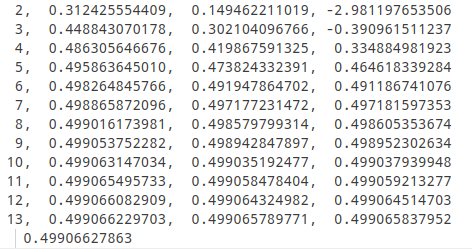
\includegraphics[width=16cm]{images/tarefa-2/tabela-1-tarefa-2.png}
\caption*{Fonte: Compilado pelo Autor.}
\label{fig:tarefa 2 - Tabela 1}
\end{figure}
